\section{Question}
Please provide documentation for a control algorithm that you developed for controlling
a real-world system. Documentation can include code snippets, system
modeling/analysis, data on system performance, and anything else that will help us
understand how you approached the problem.

\subsection *{Answer}
I will cover a part of my project on Supertruck when I worked with Daimler 2011-14. For context, the only thing changed on the system compared to the stock system was the compressor interior temperature sensors (yes, their best semi did not explicitly control interior temperature) to keep it close to stock so that they could make a business case out of this prototype.

\subsubsection * {Architecture}

\begin{figure}[h!]
  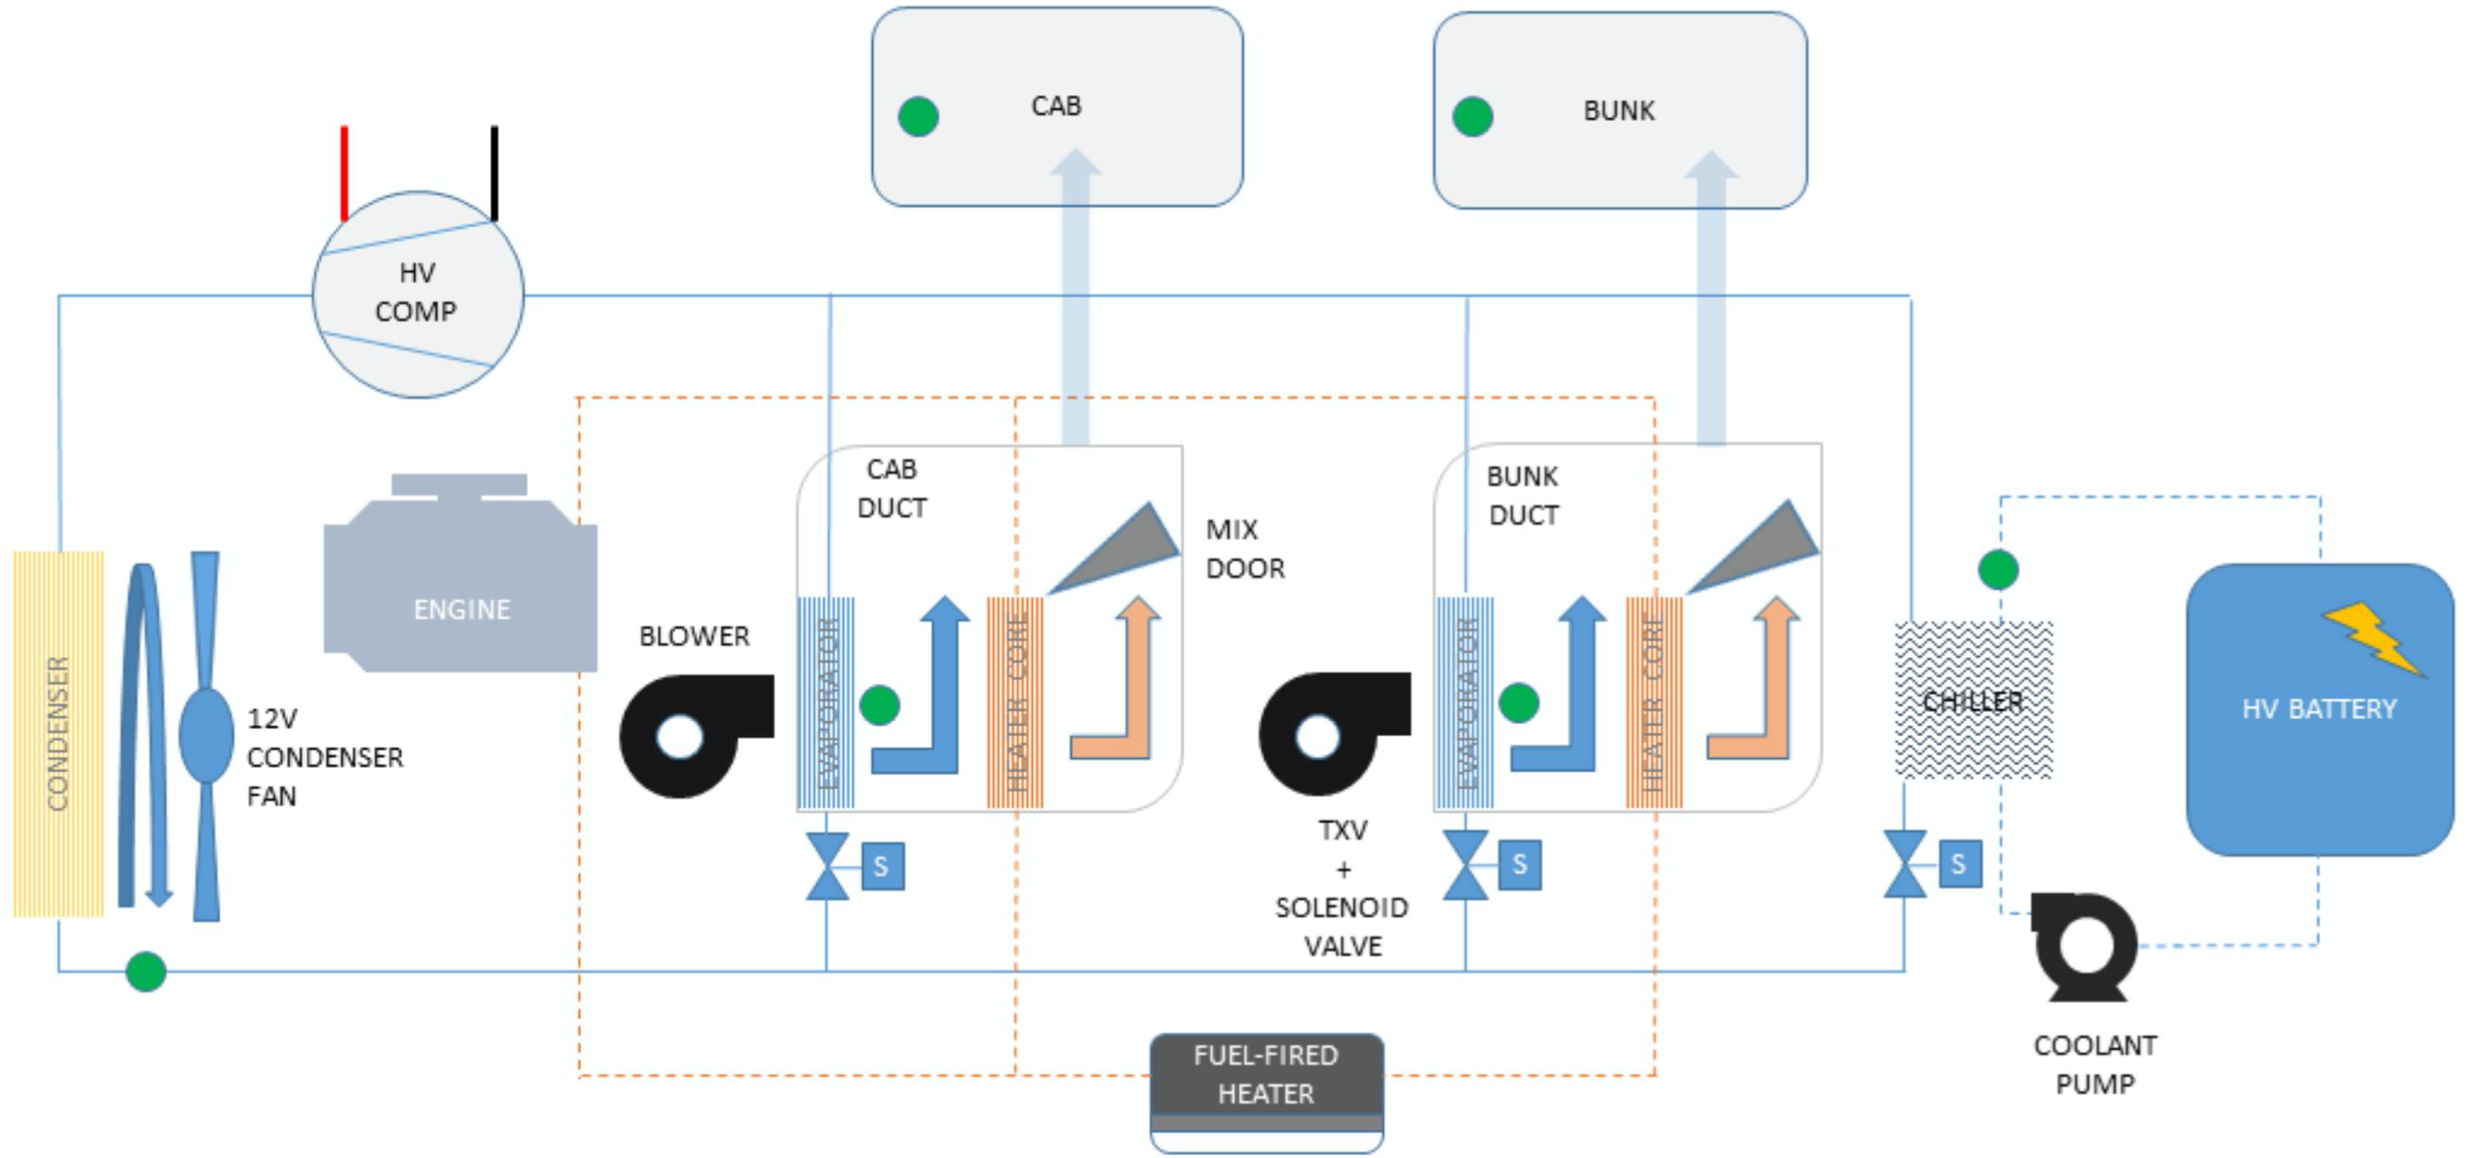
\includegraphics[width=\textwidth]{supertruck_arch}
  \caption{Supertruck Architecture}
\end{figure}

\subsubsection * {Interior Temperature Control}

The math model for the interior air is:
\begin{equation}
\dot{T} = \frac{\dot{m} C_p (T_d - T) + Q_h + Q_s + Q_{sh}}{MC_p}
\end{equation}
\newline
where:
\newline
T - interior air temperature \\
M - air mass \\
\(C_p\) - specific heat \\
\(T_d\) - duct temperature or evaporator exit air temperature \\
\(Q_h\) - human heat load \\
\(Q_s\) - cabin solar load \\
\(Q_{sh}\) - cabin-shell heat transfer \\
\\
Rearranging:
\begin{equation}
\dot{T} + \frac{\dot{m}}{M} T = \frac{\dot{m} C_p T_d + Q_h + Q_s + Q_{sh}}{MC_p}
\end{equation}

\noindent
Here are the parameters that vary:
\begin{enumerate}
  \item Blower speed - The coefficient of temperature (T) is \(\frac{\dot{m}}{M}\). That means its time constant changes with a change in \(\dot{m}\), i.e. a change in blower speed. 
  \item Air Capacitance - The cabin and bunk region can be divided from each other, or combined, depending on whether the barrier is closed or if the vehicle is in parked mode.
\end{enumerate}

As the vehicle had solenoid TXV valves, the compressor can only explicitly control one region at a time. The blower speed is set by the driver. For the interior air I created a gain-scheduled PI controller to create a target evaporator exit air temperature for the compressor.

\subsubsection * {Battery Coolant Temperature Control}
The battery coolant loop had a 4-way valve that was used for switching between a coolant-to-air HX or a coolant-to-refrigerant HX. When in the latter mode, the Hybrid Powertrain team created a requirement to control the coolant temperature to 30 \textdegree C. The compressor controlled this temperature directly.

\subsubsection * {Compressor Control}
For the following cases:
\begin{enumerate}
  \item Cabin \textbf{only} - The compressor had a gain-scheduled PI controller for controlling the evaporator exit air temperature, based on the blower speed.
  \item Chiller \textbf{only} - The compressor had a PI controller for controlling the coolant inlet temperature into the battery pack.
  \item Cabin \textbf{and} Chiller - Two controllers need to run in parallel but only one actuator, the compressor:
  \begin{enumerate}
  \item The problem is that each controller is creating a new state. The goal is to figure out which controller is 'leading' at every time step, and then get the other controller to follow for that time step.
  \item The way to do that is, at each time step, calculate the \textbf{increment} in compressor speed for each controller. If cabin controller has a higher increment, add that to the compressor speed from the previous time step. The chiller controller integrator is then set to follow the cabin controller for that time step. Reevaluate at each time step.
  \item At some point it is possible that either the cabin or the chiller could get overcooled as the compressor can only follow one of them. In that case, use the solenoid valve to shut off refrigerant. A hysteresis was used to engage/disengage the controller.
\end{enumerate}
\end{enumerate}

\noindent
Evaporator freezing - this was fortunately not a problem as the the production vehicle used a temperature sensor in the airstream in front of the evaporator instead of on the fin. For the production vehicle, the map between air temperature and freezing fin temperature had already been empirically determined. I set the minimum possible evaporator air temperature as the lower saturation limit in the cabin temperature controller.

\subsubsection * {High Side Pressure Control}
A PI controller that creates a fan speed request. The fan speed was saturated based on vehicle speed as ram air made the fan ineffective. The high side pressure target was a lookup table provided by the thermal team as a function of exterior ambient temperature.

\subsubsection * {Heating Control}
The system had a mix door that was used to control interior temperature directly. The reason is, the duct air temperature was after the evaporator but before the heater core (this was production design that we carried over), so duct air temperature control with the heater core was not possible.

Parked mode is a mode for when the vehicle is parked overnight like at a truck stop. A fuel-fired heater was turned on if required. The heater only had binary control available.

\subsubsection * {Defrost Control}
Calculate dew point temperature using exterior ambient temperature. Undercut that by a bias to ensure that air is dehumidified. Reheat air using the mix door for interior temperature control.

\subsubsection * {More on Cabin Temperature Control}
I designed the above in 2012-13. I would explore using an optimal control algo to figure the highest possible evaporator temperature during the pull down period, by using a cost function penalizing the terminal cost and control input cost. The control input cost would be the temperature delta between cabin temperature and duct temperature and have the effect of keeping the evaporator temperature as high as possible. This will save energy.

\begin{equation}
Cost \: Function \: J = fT_h^2 + \int_0^h ru^2dt
\end{equation}
where: \\
$T_h$ - Terminal (target) temperature at the end of the horizon \\
u - delta between interior and duct temperature \\
r - weight for u. This reduces the cost during the complete pull down process. \\
f - weigh for terminal temperature to ensure that system reaches target temperature
\noindent
\newline
\newline
This will allow for creating a time to reach target destination that can be changed based on subjective comfort evaluation.